
\documentclass{beamer}
\usepackage{newtxmath}
\usepackage{amsmath,amssymb}
\usepackage{tikz}
\graphicspath{{Figures/}}
\usetheme{BauhausNeuralFEM}

\title[Parent Element]{From FEM to Neural Operators: Scientific Machine Learning for Computational Mechanics\\[0.4cm]}
\subtitle{Parent Element:\\ Basis Functions, Jacobians and Gauss Quadrature}
\author{Dr-Ing Jorge Alberto L\'{o}pez Zerme\~{n}o}
\date{}

\begin{document}
{
	\usebackgroundtemplate{
		\begin{tikzpicture}[remember picture,overlay]
			\node[opacity=0.25,inner sep=0pt] at (current page.center)
			{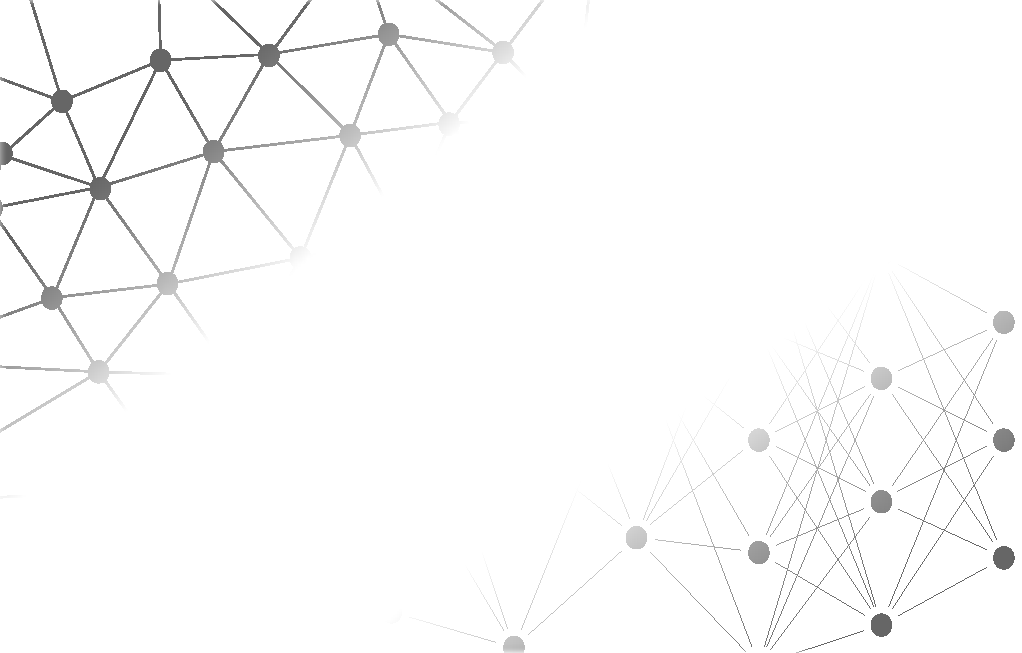
\includegraphics[width=\paperwidth,height=\paperheight]{Background.pdf}};
		\end{tikzpicture}
	}
	\begin{frame}[plain]
		\centering
		\begin{minipage}{0.21\textwidth}
			\centering
			
\includegraphics[width=\linewidth]{Bauhaus_Logo.png}
		\end{minipage}\hspace{105pt}
		\begin{minipage}{0.3\textwidth}
			\centering
			
\includegraphics[width=\linewidth]{JHU_Logo.png}
		\end{minipage}
		
		\titlepage
		\vspace{-35pt}
		Bauhaus Spring School 2026
		
	\end{frame}
}
\begin{frame}{Why a parent element?}
  \begin{itemize}
    \item Standardize on a \textbf{single reference domain}; map to real geometry.
    \item Compute shapes, derivatives, and integrals in the parent space.
    \item Clean, reusable element routines across arbitrary meshes.
  \end{itemize}
  
  \begin{center}
  	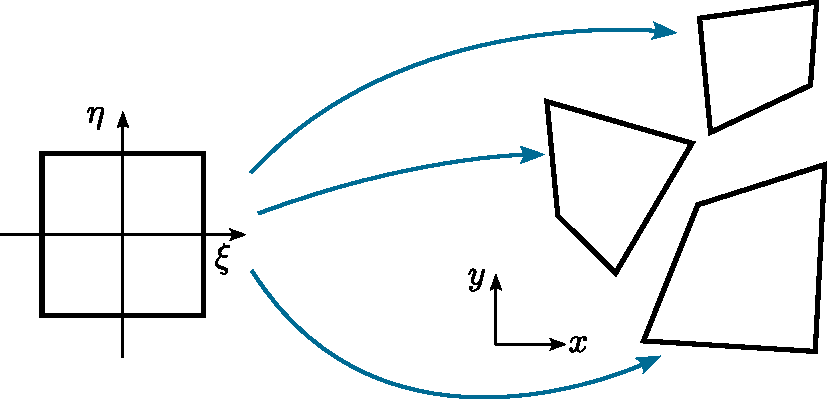
\includegraphics[width=0.6\linewidth]{Figures/Parent_Element.pdf}
  \end{center}
  
\end{frame}
\begin{frame}{1D Lagrange bases ($\xi\in[-1,1]$)}
  \begin{block}{General formula}
    \[ N_a(\xi)=\prod_{b\neq a}\frac{\xi-\xi_b}{\xi_a-\xi_b},\quad N_a(\xi_b)=\delta_{ab} \]
  \end{block}
  
  \begin{minipage}{0.47\textwidth}
  	\begin{block}{\footnotesize Linear Basis Functions ($p=1$)}
  		\footnotesize
  		\begin{array*}
  			N_1 &=\tfrac{1-\xi}{2} \\
  			N_2 &=\tfrac{1+\xi}{2} \\
  			&
  		\end{array*}
  		
  		\vspace{3pt}
  		\begin{center}
  			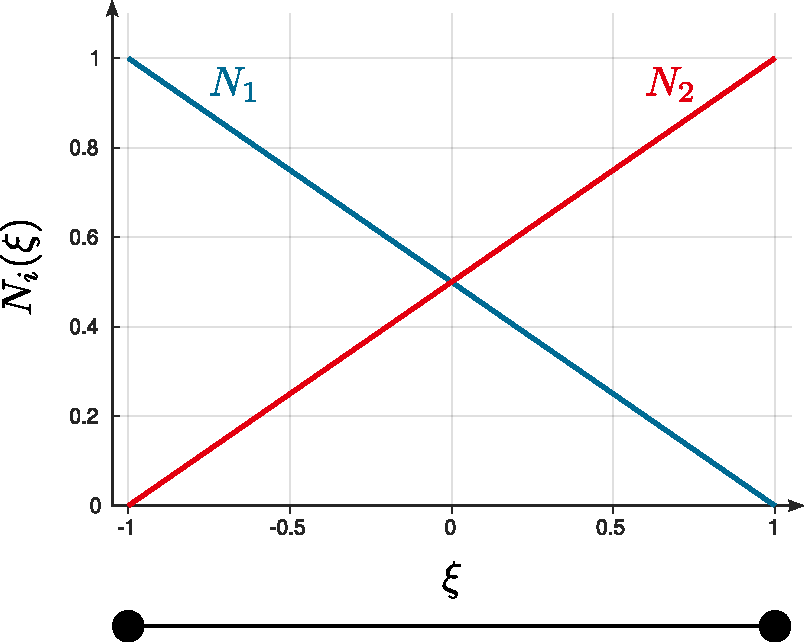
\includegraphics[width=0.8\linewidth]{Figures/lagrange1D_linear.pdf}
  		\end{center}
  	\end{block}
  \end{minipage}\hfill
  \begin{minipage}{0.47\textwidth}
  	\begin{block}{\footnotesize Quadratic Basis Functions ($p=2$)}
  		\footnotesize
  		\begin{array*}
  			N_1 &=\tfrac12\,\xi(\xi-1) \\ 
  			N_2 &=1-\xi^2 \\
  			N_3 &=\tfrac12\,\xi(\xi+1)
  		\end{array*}
  		
  		\vspace{3pt}
  		\begin{center}
  			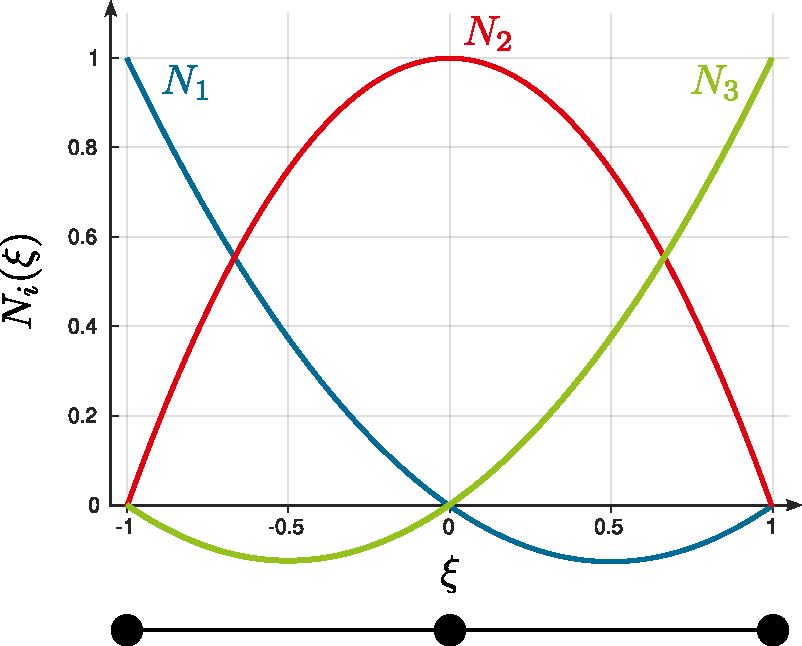
\includegraphics[width=0.8\linewidth]{Figures/lagrange1D_quadratic.pdf}
  		\end{center}
  		
  	\end{block}
  \end{minipage}

\end{frame}


\begin{frame}{1D isoparametric mapping}
	\footnotesize
	\begin{minipage}{0.4\textwidth}
		\begin{center}
			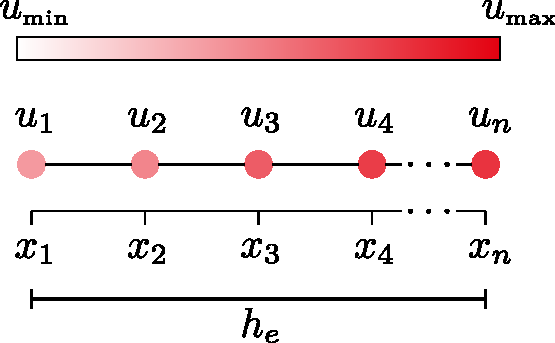
\includegraphics[width=\linewidth]{Figures/Isoparametric_1D.pdf}
		\end{center}
	\end{minipage}\hfill
	\begin{minipage}{0.5\textwidth}
		\footnotesize
		\begin{itemize}
			\item Same $N_i$ for interpolating $x(\xi)$ and $u(\xi)$
		\end{itemize}
		\[ x(\xi)=\sum_i N_i x_i,\quad  u(\xi)=\sum_i N_i u_i, \]
		\begin{itemize}
			\item Jacobian: Represents how $d\xi$ scales into $dx$
		\end{itemize}
		\[J=\frac{dx}{d\xi}=\sum_i x_i N_i' \quad \frac{du}{dx}=\frac{1}{J}\sum_i u_i N_i' \]
	\end{minipage}
  
  \vspace{20pt}
  The Jacobian $J(\xi)$ corrects the integral over $\xi$, so we still integrate over the physical length $x$.
  \begin{itemize}
    \item Integral: $\displaystyle \int g(x)\,dx=\int g(x(\xi))\,J(\xi)\,d\xi$
    \item Check: $J(\xi)>0$
  \end{itemize}
\end{frame}


\begin{frame}{Q4 Element}
	\begin{minipage}{0.4\textwidth}
		\begin{center}
			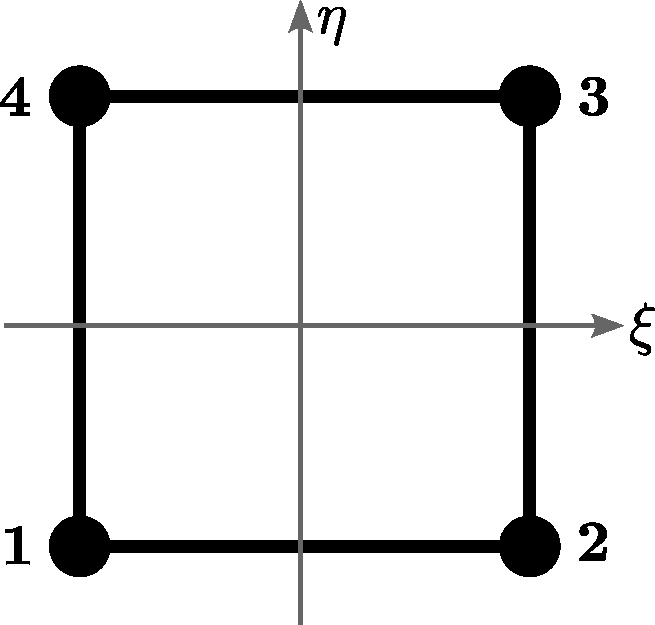
\includegraphics[width=0.55\linewidth]{Figures/Parent2D_Numbering.pdf}
		\end{center}
		\footnotesize
		\[
		\begin{aligned}
		N_1&=\tfrac14(1-\xi)(1-\eta),\\
		N_2&=\tfrac14(1+\xi)(1-\eta),\\
		N_3&=\tfrac14(1+\xi)(1+\eta),\\
		N_4&=\tfrac14(1-\xi)(1+\eta)
		\end{aligned}
		\]
		\[ x(\xi,\eta)=\sum N_i x_i,\; y(\xi,\eta)=\sum N_i y_i \]
		\[
		\mathbf{J}=
		\begin{bmatrix}
		\sum x_i\,\partial_{\xi} N_i & \sum y_i\,\partial_{\xi} N_i\\
		\sum x_i\,\partial_{\eta} N_i & \sum y_i\,\partial_{\eta} N_i
		\end{bmatrix},
		\]
		\[\det\mathbf{J}>0\]
		
	\end{minipage}\hfill
	\begin{minipage}{0.53\textwidth}
		\begin{center}
			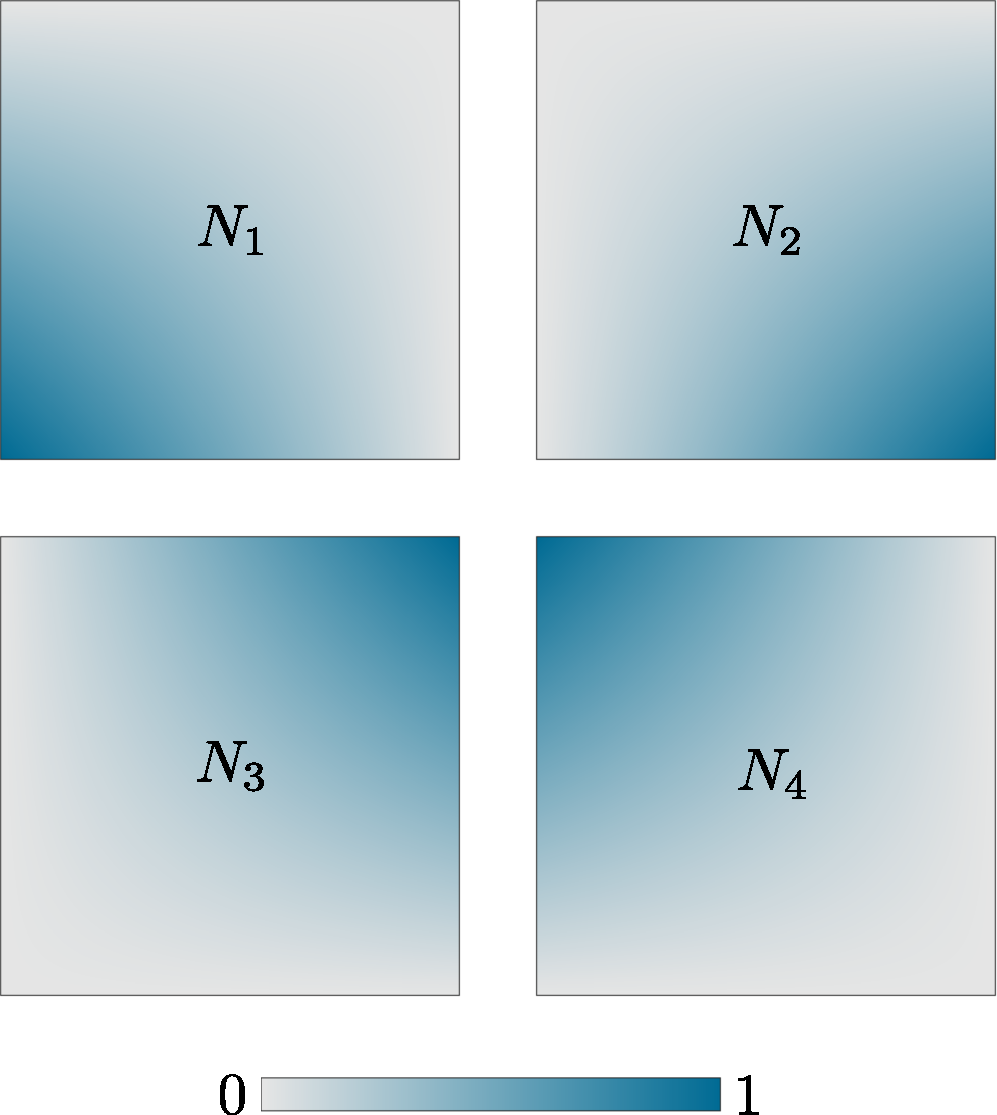
\includegraphics[width=\linewidth]{Figures/Basis2D.pdf}
		\end{center}
	\end{minipage}
\end{frame}

\begin{frame}{Physical gradients via chain rule}
	\footnotesize
	\begin{center}
		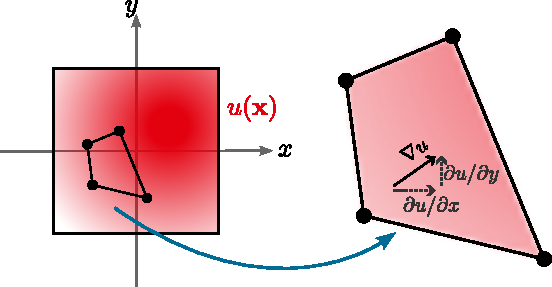
\includegraphics[width=0.65\linewidth]{Figures/Physical_Gradients_2D.pdf}
	\end{center}
	
  \[ \nabla_{\!\mathbf{\xi}}N_i=\begin{bmatrix}\partial_\xi N_i\\ \partial_\eta N_i\end{bmatrix},\quad
     \nabla N_i=\mathbf{J}^{-1}\nabla_{\!\mathbf{\xi}}N_i,\quad
     \nabla u=\sum_i \nabla N_i\,u_i \]
     \begin{itemize}
     	\item $\mathbf{J}$ maps small parent areas to physical areas: \\
     	$d\Omega = \vert\mathbf{J}\vert d\xi d\eta$ $\Rightarrow$ $\displaystyle \iint g\ \det\mathbf{J}\,d\xi\,d\eta$
     	\item $\mathbf{J}^{-1}$ maps parent gradients to physical gradients: $\nabla = \mathbf{J}^{-1}\nabla_{\xi}$
     	\item Avoid near-zero $\det\mathbf{J}$ (distortion)
     \end{itemize}

\end{frame}


\begin{frame}{Gauss--Legendre on $[-1,1]$}
	\small
	\[ \int_{-1}^{1} f(\xi)\,d\xi \approx \sum_k w_k f(\xi_k),\quad
	\int g(x)\,dx \approx \sum_k w_k\,g(x(\xi_k))\,J(\xi_k) \]
	\begin{minipage}{0.7\textwidth}
		\small
		\begin{itemize}
			\item 1-pt: $\xi=\{0\}$, $w=\{2\}$
			\item 2-pt: $\xi=\{\pm 1/\sqrt{3}\}$, $w=\{1,1\}$
			\item 3-pt: $\xi=\{0,\pm\sqrt{3/5}\}$, $w=\{8/9,5/9,5/9\}$
		\end{itemize}
	\end{minipage}\hfill
	\begin{minipage}{0.28\textwidth}
		\begin{center}
			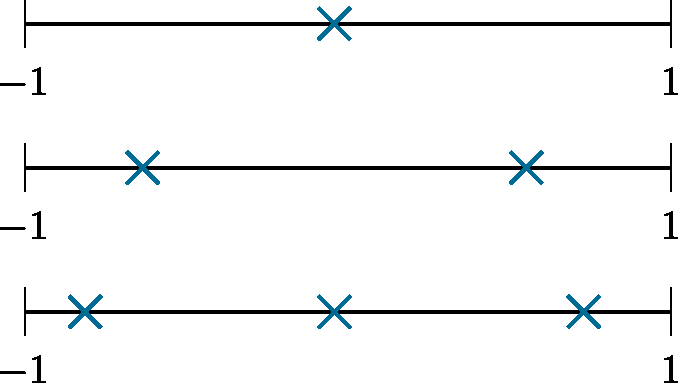
\includegraphics[width=\linewidth]{Figures/Gauss_Points_1D.pdf}
		\end{center}
	\end{minipage}
  
  	\[ \hspace{-15pt}\iint f(\xi,\eta)\,d\xi\,d\eta \approx \sum_{k,\ell} w_k w_\ell\, f(\xi_k,\eta_\ell), \quad  \int_{\Omega_e} \hspace{-6pt}g\,d\Omega \approx \sum_{k,\ell} w_k w_\ell\, g(\xi_k,\eta_\ell)\,\det\mathbf{J}(\xi_k,\eta_\ell) \]
  	
  	\begin{center}
  		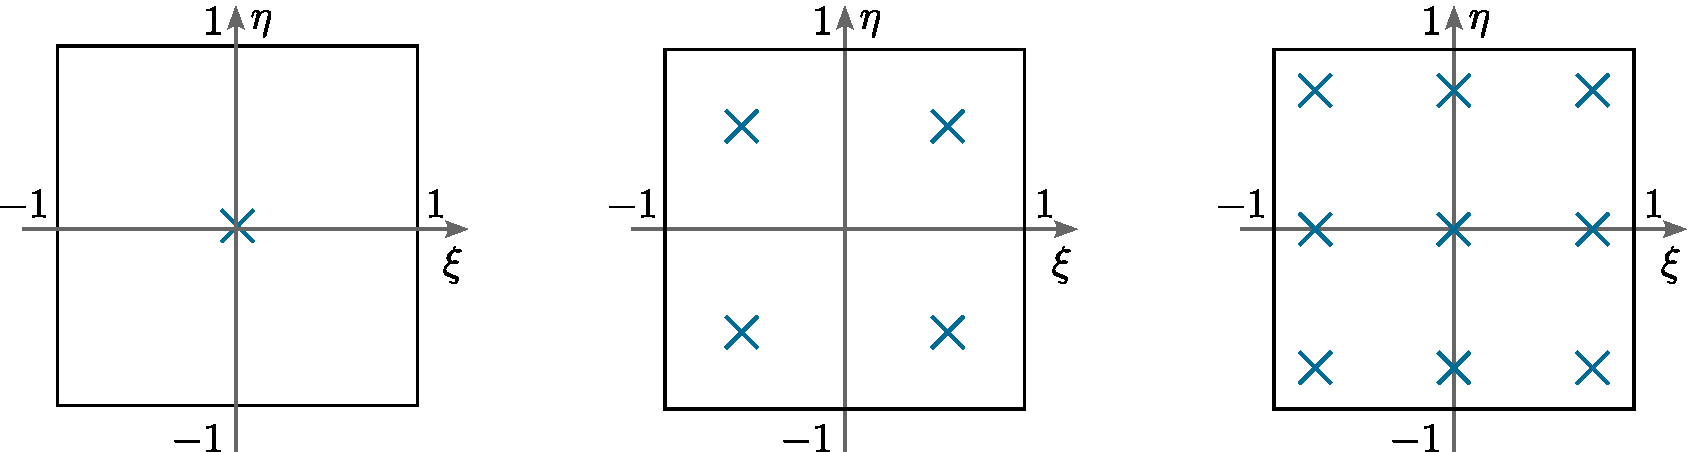
\includegraphics[width=0.85\linewidth]{Figures/Gauss_Points_2D.pdf}
  	\end{center}
\end{frame}



\begin{frame}{Summary and outlook}
	\small
	\textbf{Engineering checks}
	\begin{itemize}
		\item Check $\det \mathbf{J}(\xi,\eta) > 0$ on every element (no inverted elements).
		\item Quadrature: choose Gauss order so that the rule is exact for the
		polynomial degree of the integrand.
		\item Mesh quality: avoid elements with very small $|\det \mathbf{J}|$ or very large $\|\mathbf{J}^{-1}\|$.
		\item Reuse the same parent-element, $\mathbf{J}$, and quadrature routines for all elements.
	\end{itemize}
	
	\vspace{0.6em}
	\textbf{Relevance for PINNs and Neural Operators}
	\begin{itemize}
		\item The same parent-element mapping and Jacobian appear when evaluating PDE residuals at quadrature points.
		\item In weak-form / variational PINNs, domain and boundary integrals in the loss use exactly these $\,\mathbf{J}$ and Gauss rules.
		\item Othe scientific computing approaches are often trained on FEM data computed with these interpolation and quadrature choices.
	\end{itemize}
\end{frame}

\end{document}
